\documentclass[a4j]{jarticle}
\usepackage{graphicx}
\usepackage{jcfd39}
\usepackage{url}
%
%\usepackage{ulem} %proofreading e.g. \uuline{ \uwave{  \sout{demo}}}
%
%\makeatletter  % Change the style of citation and biblabal - II
%\def\@cite#1{$^{\mbox{\scriptsize{(#1})}}$}
%\makeatother

\newcommand{\ctext}[1]{\raise0.2ex\hbox{\textcircled{\scriptsize{#1}}}}


%%\def\papernum{講演番号}                %講演番号を記して下さい

\title{日本語タイトル $<$14pt ゴシック,Arial$>$}   %和文タイトルを記して下さい
\etitle{English Title $<$12 pt Arial$>$}   %英文タイトルを記して下さい

                                    %和文著者名を記して下さい
\author{\begin{tabular}{cl}
$\bigcirc$ & 著者1,所属機関略称, 
             所属機関所在地, 
             E-mail:
             $<$10pt,明朝体,Times$>$ \\
           & 著者2,所属機関略称,
             所属機関所在地, 
             E-mail:
\end{tabular} }

                                    %英文著者名を記して下さい
\eauthor{\begin{tabular}{l}
    Author1, 
    Affiliation, 
    Address \\
    Author2, 
    Affiliation, 
    Address
\end{tabular} }

                                    %アブストラクトを記して下さい
\abstract{%
%
    Abstract must be 100 -- 150 words using 9pt Times font.
    This is a simple example of how to prepare the paper for CFD39.
    The headings should appear as above.
    The instruction is written in the main body.
    Abstract must be 100 -- 150 words using 9pt Times font.
    This is a simple example of how to prepare the paper for CFD39.
    The headings should appear as above. The instruction is written in the main body. 
%
}
\begin{document}
\baselineskip=1zw
\maketitle
                                    %ここから本文です

\section{提出物}

\vspace*{2mm}
講演論文(PDFファイル): A4版2段組,1--10ページ,10MB以内.
\vspace*{2mm}

講演論文のPDFファイルは,以下のようにして作成して下さい. Word, TeX 等の適当なソフトウェアを用いて図表すべてを貼り込んだ原稿を作成し,PDFファイルに変換して下さい.フォントは可能な限り埋め込み,印刷サイズがA4であることを確認してください.作成したPDFファイルについては,できる限り,複数のPC上で文字化け等が発生しないか確認の上,ご提出下さい.


\section{原稿用紙}

A4 版の白紙の上下に20 mm,左右に15 mm の余白をとり,本文は原則として9ポイントの文字を使用して印字して下さい.また,表題・著者名等の部分を除いて2段組みで作成して下さい.


\section{体裁} %(講演予稿)q

\begin{enumerate}
    \item[・] ヘッダー:
        ヘッダーは変更しないでください.
    \item[・] 邦文表題:
        14ポイント・ゴシック体, Arial フォントで用紙中央に印字する.
        なお,表題,著者名の変更はできません.
    \item[・] 英文題目:
        12ポイント・Arial, Helvetica, cm(bold)フォントで用紙中央に印字する.
        Main Words の最初の文字のみ大文字とする.
    \item[・] 邦文著者名:
        10ポイント・明朝体で英文題目との間を1行空け,著者氏名と所属機関名略称,所在地,(可能ならば)E-mail アドレスを書く.
    \item[・] 英文著者名:
        10ポイント・Times, Times New Roman, cm フォントを用い,英文で著者名,所属機関名,所在地を書く.
    \item[・] 英文要旨:
        9ポイント・Times, Times New Roman, cm フォントを用い,英文著者名との間を1 行空け,
        100--150words程度の英文要旨を幅150mm に収まるように印字する.
    \item[・] 本文:
        英文要旨との間を1 行空けて書き始める.
    \item[・] 図表:
        鮮明かつ適当な大きさのものを適当な位置に貼付する.
        図表中の文字及び表題,キャプションは英文とする.
\end{enumerate}


\begin{figure}[b]
    \vspace*{-5mm}
    \begin{center}
%       bmpファイルを貼り込む例です
%       \includegraphics[bb=0 0 400 280, width=0.7\linewidth]{pte.bmp}
        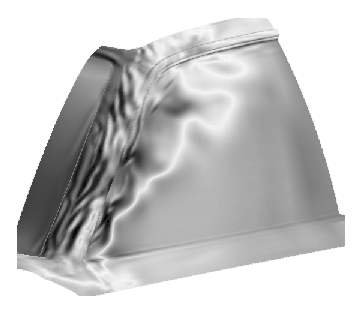
\includegraphics[width=0.32\textwidth,clip]{sample.eps}
    \end{center}
    \caption{Sample figure.}
    \vspace*{-5mm}
\end{figure}

\begin{enumerate}
    \item[・] 文献:
        例えば, この$^{(1)}$ように引用し, 末尾にまとめる.
\end{enumerate}

\section{別刷り等}

シンポジウム参加者に電子版を配布します.別刷りは作成されません.

\section{原稿提出先}

\begin{enumerate}
    \item[(1)] 
    講演論文のPDFファイルは,ホームページに記載されている方法に従いご提出下さい.
    \item[(2)]
    原稿に関する問い合わせは,下記までE-mailにてお願いいたします.\\
E-mail: cfd39@nagare.or.jp\\
(第39回数値流体力学シンポジウム事務局)

\end{enumerate}

\section{流体力学会誌「ながれ」への再投稿}
本シンポジウムの講演予稿の流体力学会誌「ながれ」への再投稿を希望する場合は,
シンポジウム終了後に,「講演予稿のPDFファイル」に「ながれ投稿票(CFDシンポ用)$\!\!$」を添えて,
日本流体力学会事務局(info@nagare.or.jp)まで投稿してください
(ながれ投稿票(CFDシンポ用)$\!\!$)の書式はホームページよりダウンロードして下さい).

なお,投稿される前に,「ながれ」の投稿規定をご一読願います.
査読は「ながれ」編集委員会で行われますので,査読後の修正等は編集委員会からの指示に従ってください.
掲載可となった場合は,「ながれ」のテンプレートを用いた最終原稿の体裁書き直しの指示があります.
その他については,下記の「日本流体力学会」「ながれ」のホームページに掲載してある内容に準拠するものとします.

\noindent
【参考ホームページ】\\
\url{http://www.nagare.or.jp/} \\
\url{http://www.nagare.or.jp/nagare/nagare_index.html}

\section*{参考文献}

\begin{enumerate}
    \item 荒川,谷口, ``論文の書式について,'' 第17回数値流体力学講演論文集, 1 (2003), pp. 1-1.
    \item Arakawa, C. and Taniguchi, N., ``How to prepare the paper,'' Proc. 17th CFD Symp., 1 (2003), pp. 1-1.
\end{enumerate}

\end{document}
